\subsection{Overview: High-level components and their interaction}
This chapter describes the system components both at the physical and logical level.
The main high level components of the system are the following:
\begin{itemize}
\item
\textbf{Database:} The database server which is responsible for the data storage and retrieval. It doesn’t implement any logic as it is used only for data storing purposes. This layer must guarantee that the ACID properties are respected.
\item
\textbf{Application server:}  The application server contains all the logic on the server side of the system. This layer implements RESTful APIs and is used for registrations, login, backup and restore purposes.
\item
\textbf{Mobile Application:} The application consists in the client side of the application. It is installed on the users’ devices and implements most of the logic of the system. 
For the account/backup purposes it communicates directly with the application server, while for all the other functions is standalone.
\end{itemize}
The components are structured in a three layer application, shown in the following figure.
\begin{figure}[!h]
\centering
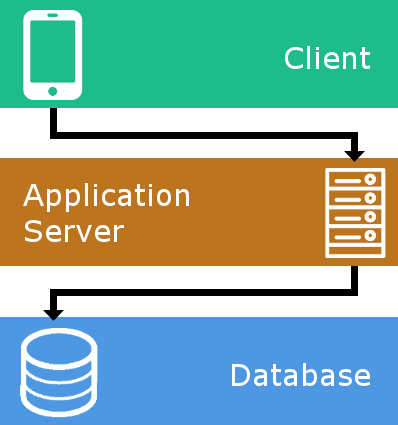
\includegraphics[scale=0.8]{images/highlevelstructure}
\caption{High Level Structure}
\label{ref:highlevelstructure}
\end{figure}

\clearpage
\subsection{Component View}
\subsubsection{High-Level Component View}
\begin{figure}[!h]
\centering
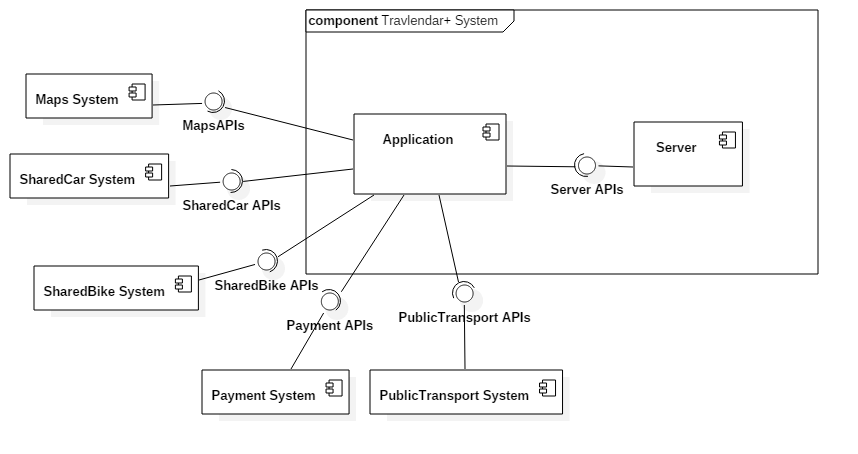
\includegraphics[scale=0.4]{images/ComponentDiagramSystem}
\caption{High Level Component View}
\label{ref:highlevelcomponentview}
\end{figure}
Component to be developed:
\begin{itemize}
\item
\textbf{Application:} It is the core of the system, it manages all information provided by the others services and performs the majority of the functions. It provides the client access to the entire system.
\item
\textbf{Server:} This component has a backup role. It receives the data from the application and provides them when necessary (e.g. during the login operation).
\end{itemize}
Component to be integrated in the system:
\begin{itemize}
\item
\textbf{MapsSystem:} It is the provider of the maps and all necessary information for the computation of the journey.
\item
\textbf{SharedCarSystem, SharedBikeSystem:} Those component provide all information (availability, location and costs) respectively shared cars and shared bikes.
\item
\textbf{PublicTransportSystem:} It provides all information about the public transport of the city.
\item
\textbf{WeatherSystem:} It provides the weather forecasts in the city.
\item
\textbf{PaymentSystem:} This component provides the payment service.
\end{itemize}

\clearpage
\subsubsection{Application System}
\begin{figure}[!h]
\centering
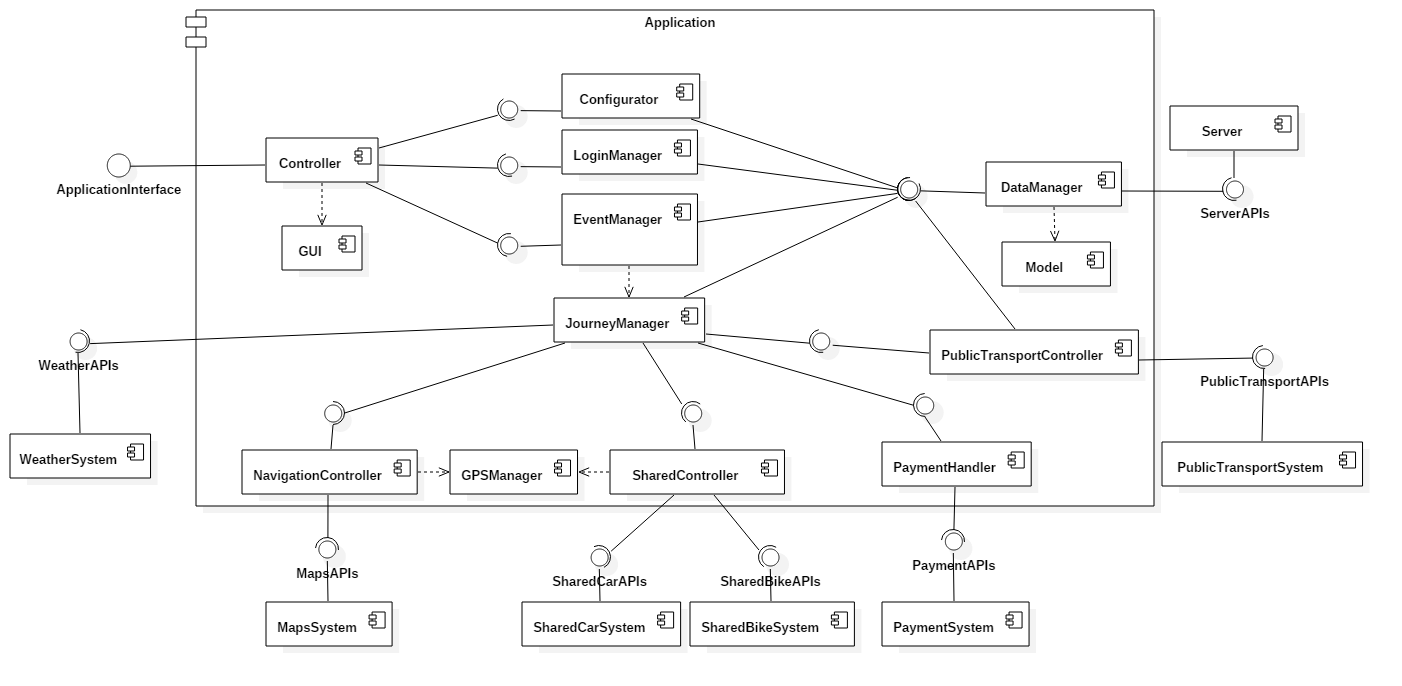
\includegraphics[scale=0.35]{images/ComponentDiagramApplicationSystem}
\caption{Application Component Diagram}
\label{ref:componentdiagramapplicationsystem}
\end{figure}
\begin{itemize}
\item
\textbf{NavigationController:} The component that provides navigation utilities using the Maps APIs and GPS.
\item
\textbf{GPSManager:} The component that handles and gives the GPS information.
\item
\textbf{SharedController:} The component that provides information of all shared systems.
\item
\textbf{PaymentHandler:} The component that handles the payment operations to buy a ticket for a public transport. It ensures that the user is able to successfully complete the payment.
PublicTransportController: The component manages the availability information and the timetable of all public transport.
\item
\textbf{DataManager:} The component that implements and provides through an appropriate interface the methods for accessing the data of our system and it takes care to send the data to the server.. This intermediate component between the entities of the the model and the other components will facilitate extendibility.
\item
\textbf{Model:} It represent how the data are structured (specified in distinct diagram) in the application and ready to be stored by the server on the database.
\item
\textbf{LoginManager:} The component that handles the login operation.
\item
\textbf{Configurator:} The component that offers the configuration functionalities
to customize a set of parameters of the user account.
\item
\textbf{Event Manager:} The component that handles the operations to create and manage an event.
\item
\textbf{Journey Manager:} It manages the user journey.
\item
\textbf{View Controller:} The component that handles the update of the GUI and the retrieval of the user input through the interface.
\item
\textbf{GUI:} Implementation of the presentation layer of the application.
\end{itemize}

\subsubsection{Server System}
\begin{figure}[!h]
\centering
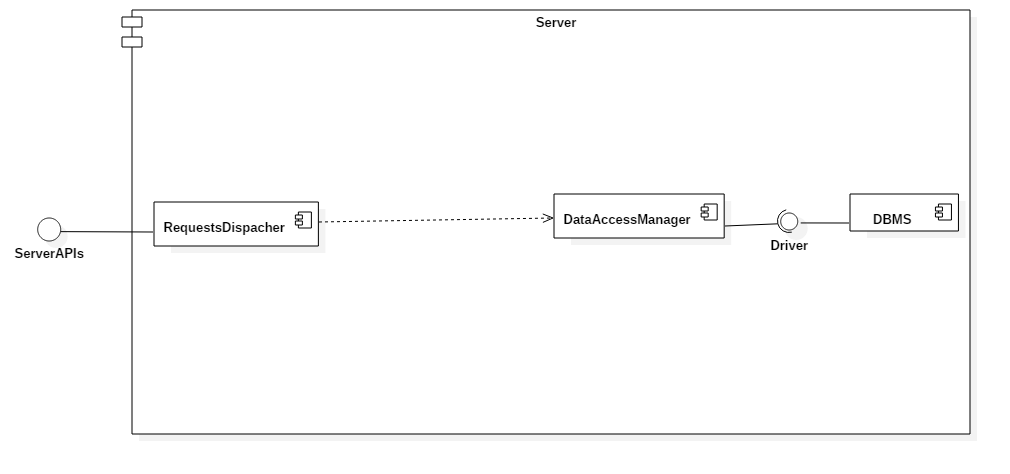
\includegraphics[scale=0.4]{images/ComponentDiagramServer}
\caption{Server Component Diagram}
\label{ref:componentdiagramserver}
\end{figure}
\begin{itemize}
\item
\textbf{RequestDispatcher:} It handles the requests from the application.
\item
\textbf{DataAccessManager:} The component that manages access to the database using a specific driver.
\item
\textbf{DBMS:} The system that will take care of the management of the data, integrated in our system using a specific driver.
\end{itemize}


\clearpage
\subsection{Deployment View}
This diagram purpose is to show the hardware components of our system and where the code is going to run.
\begin{figure}[!h]
\centering
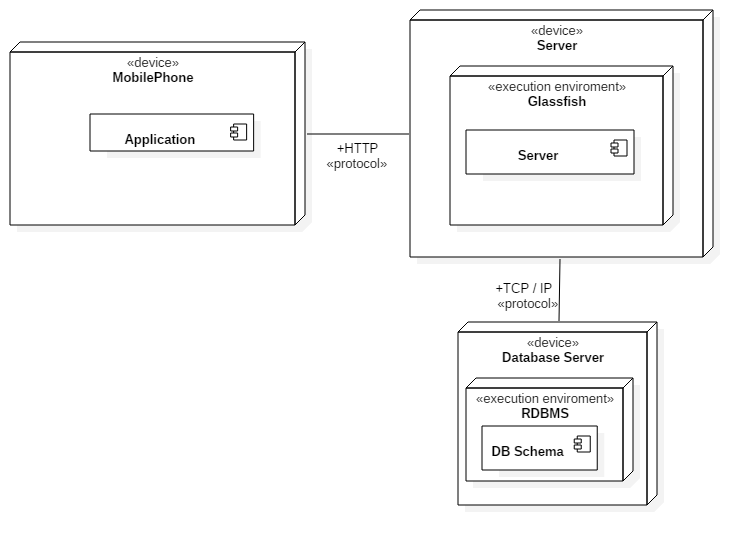
\includegraphics[scale=0.4]{images/DeploymentDiagram}
\caption{Deployment Diagram}
\label{ref:deploymentdiagram}
\end{figure}

\clearpage
\subsection{Runtime View}

\subsubsection{Visitor Registration}
\begin{figure}[H]
\centering
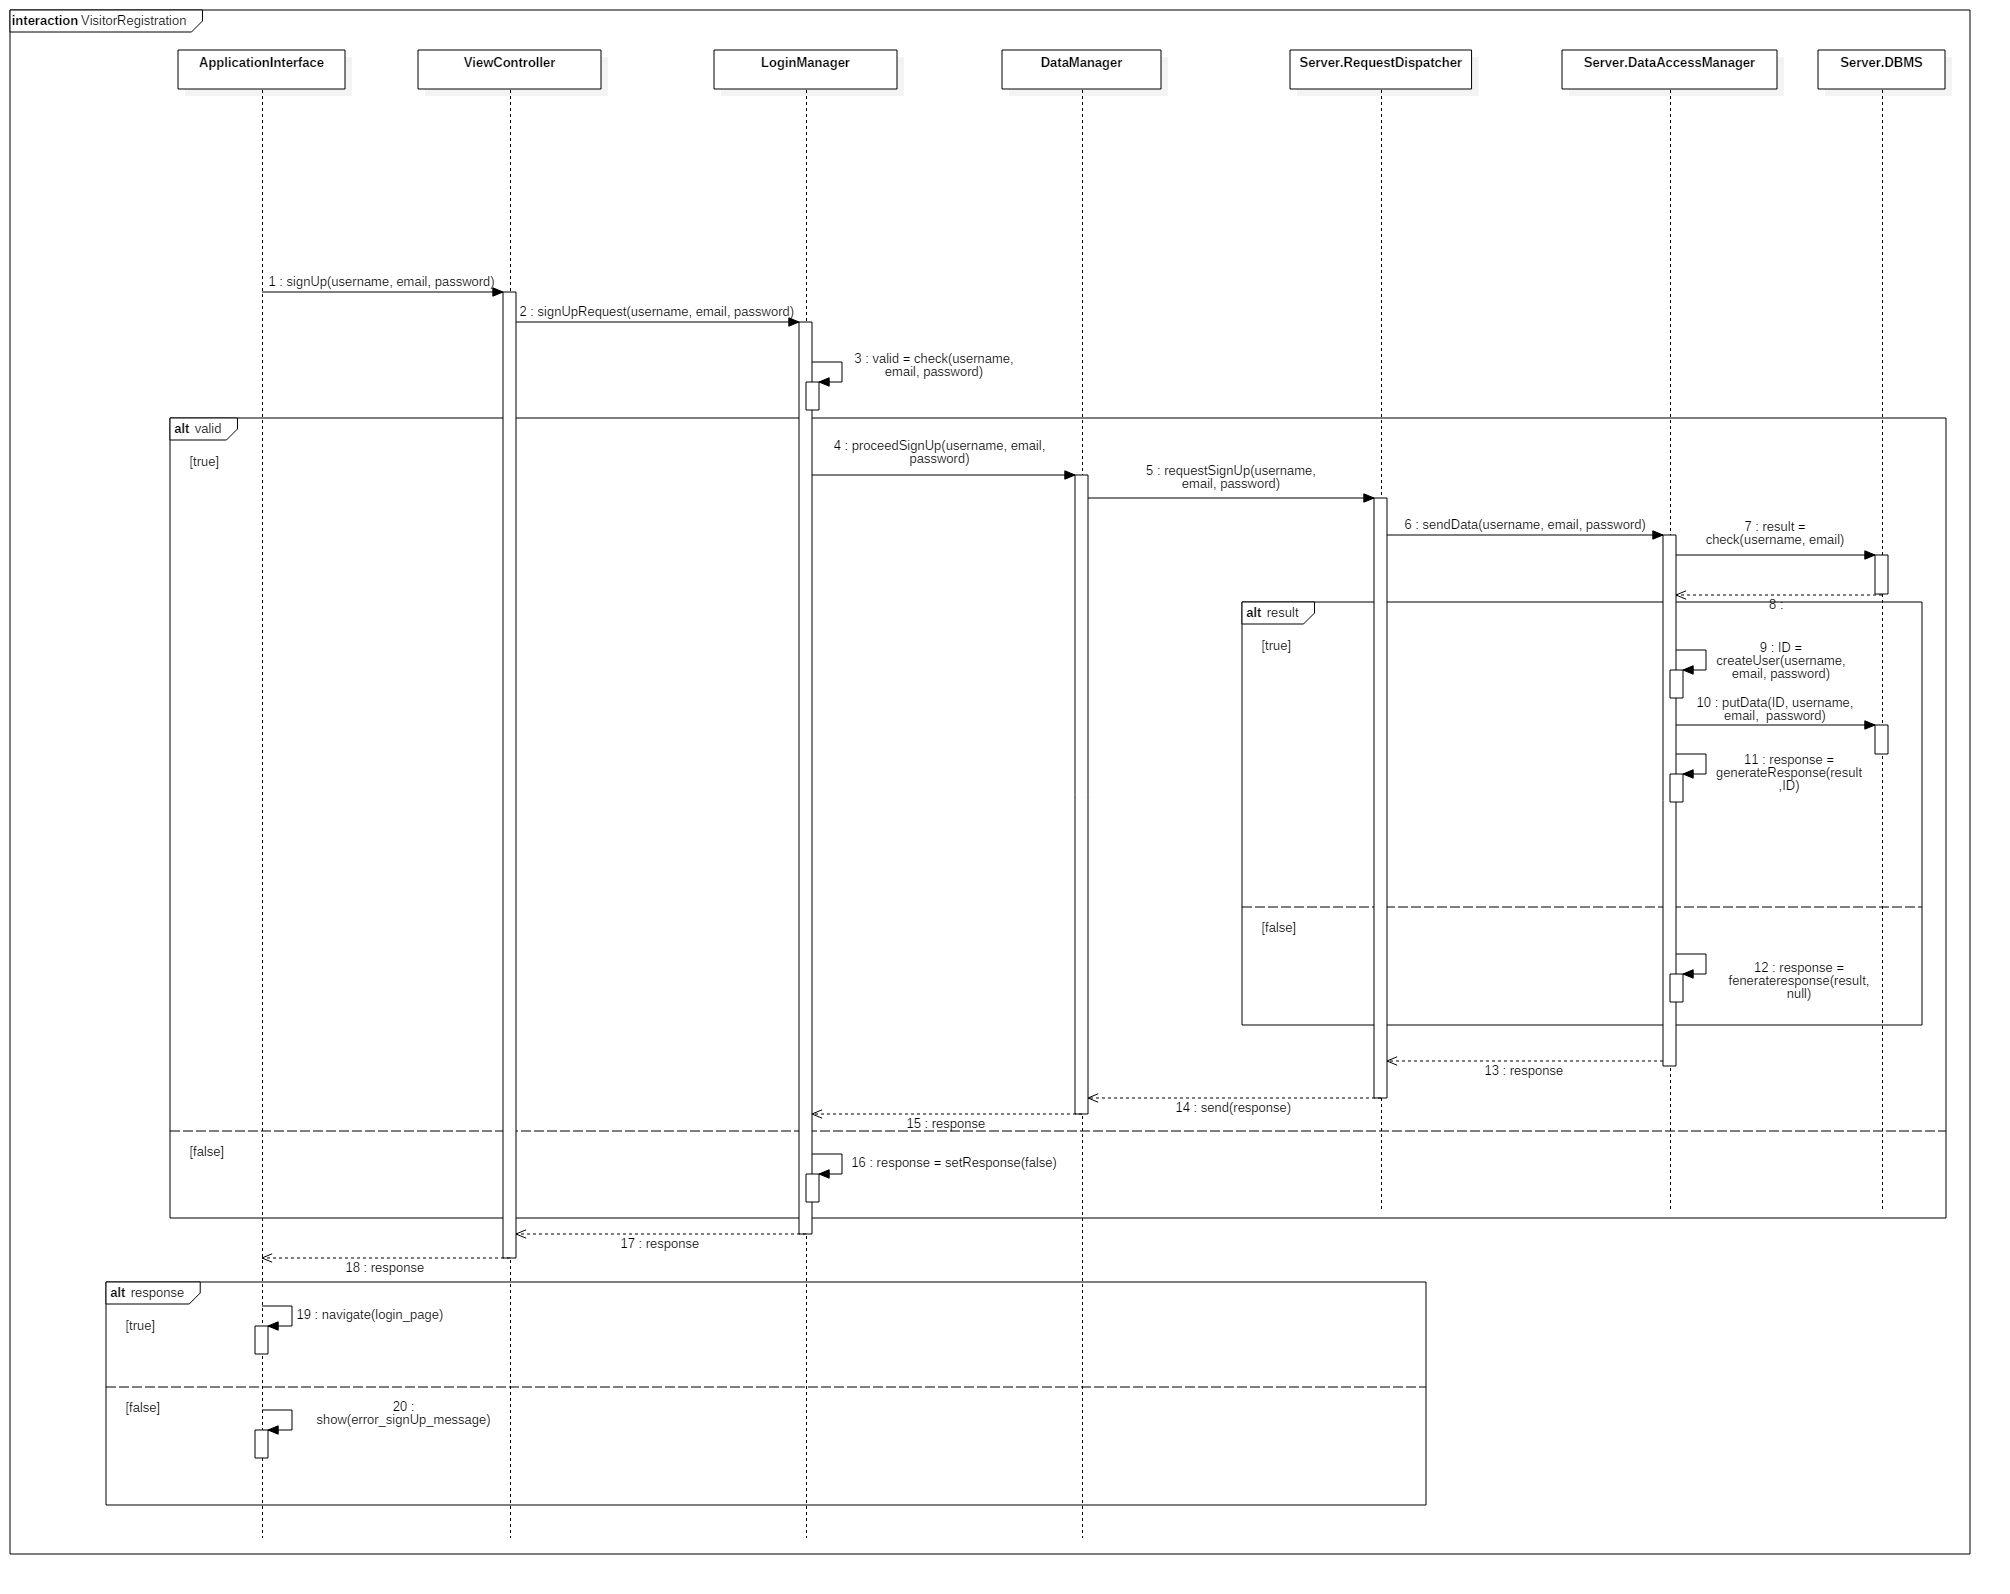
\includegraphics[scale=0.25]{images/VisitorRegistration}
\caption{Visitor Registration}
\end{figure}In this runtime diagram you can see the registration process on the application. The informations are sent by the MobileApplication to the ViewController that send thirs to the specific manager, in this case the LoginManager. The LoginManager send the information to the DataManager and it check with the Model if the username or the email are already in use or not. The answer return from model to the LoginManager, in case of positive answer the LoginManager create an ID for the user and send all data to the DataManager that it put theirs in the Model and generate a positive response; in case of negative answer, the LoginManager generate a negative response. The response is passed to the MobileApplication that show a confirm or error dialog respectively in case of positive or negative response.

\subsubsection{Login User}
\begin{figure}[H]
\centering
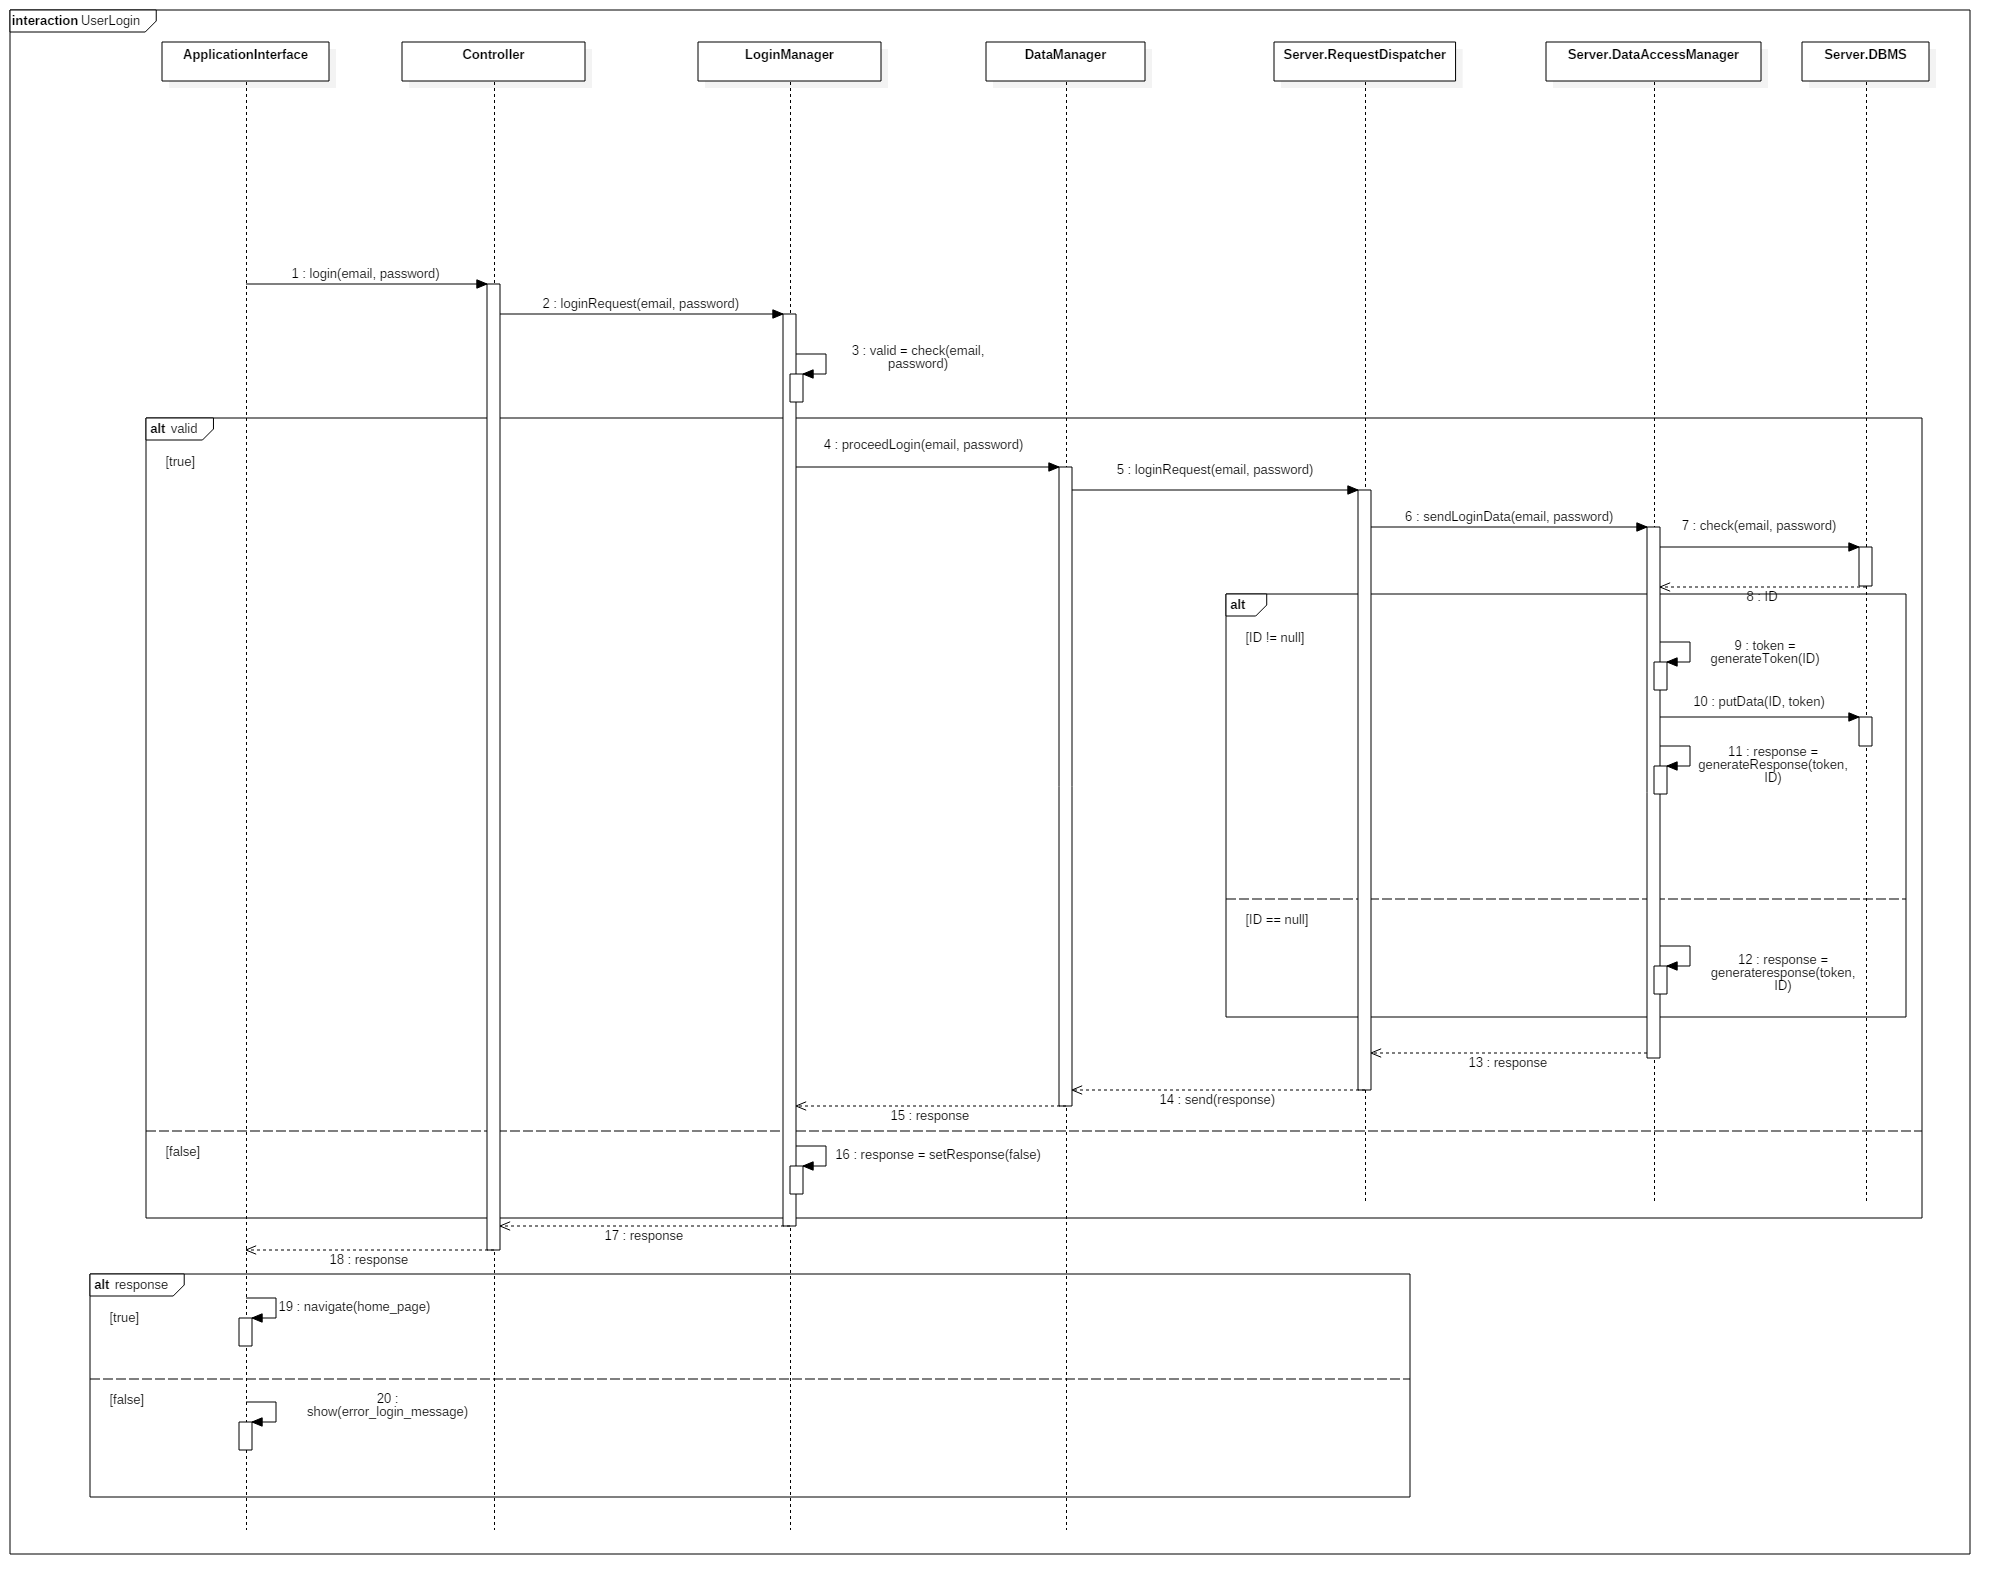
\includegraphics[scale=0.25]{images/UserLogin}
\caption{Login User}
\end{figure}In this runtime diagram you can see the login process for a user that is already registered in the application. The login informations are sent by the ApplicationInterface to the ViewController that calls the LoginManager that checks if the parameters are typed correctly. If the parameters are not valid the LoginManager generates a negative response, if it is valid you can proceed with the login process and pass the data to the DataManager that makes a request to the server. The RequestDispatcher on the server manages the requests and checks the data in the DBMS passing by the DataAccessManager. In case of the data are present in the DBMS, the DataAccessManager generates a token and put this in the DBMS and after it generates a positive response; in case of the data are not present the DataAccessManager generates a negative response. In base of positive or negative response the ApplicationInterface show respectively the home page or an error message.

\subsubsection{Setup Preferences}
\begin{figure}[H]
\centering
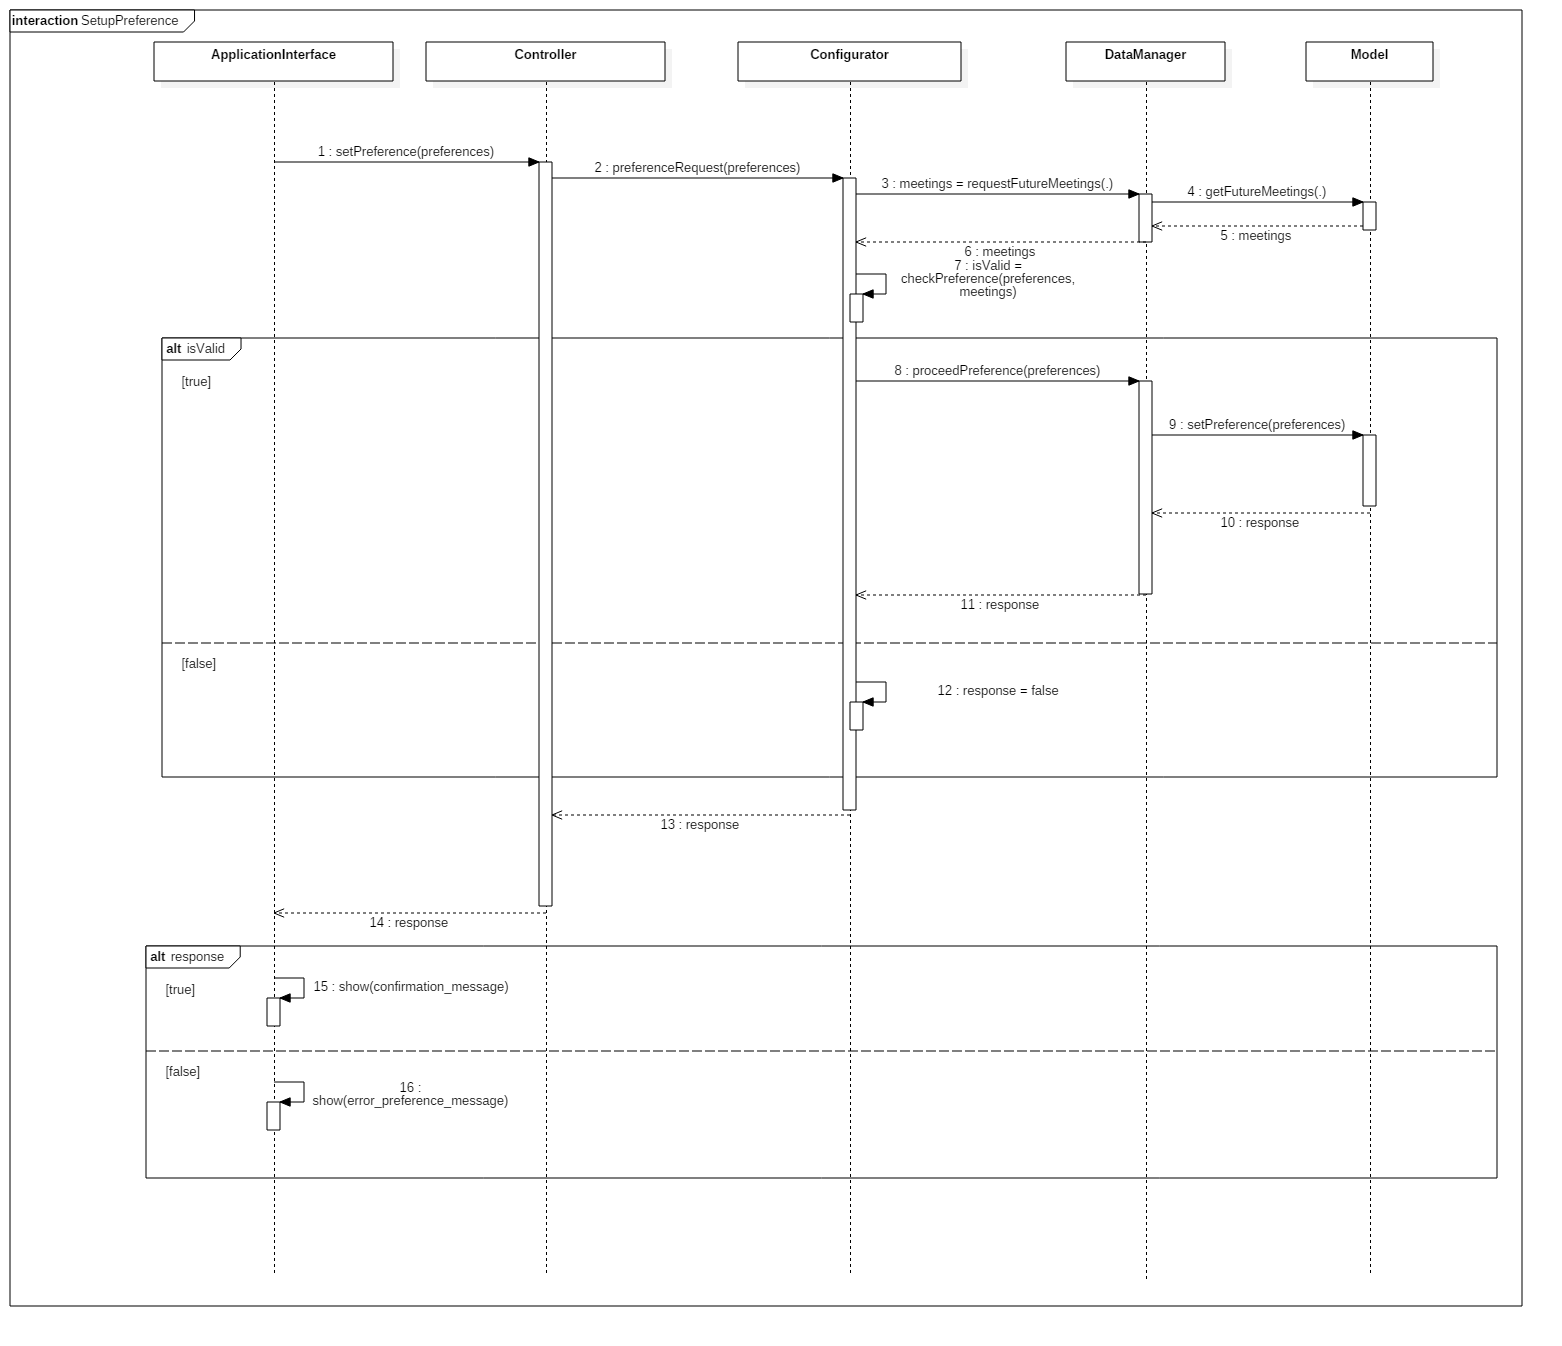
\includegraphics[scale=0.25]{images/SetupPreference}
\caption{Setup Preferences}
\end{figure}This diagram shows how the user can set your preferences in Travlendar+ application. The ApplicationInterface gives the all preferences setted by the user, to the ViewController that makes a request to the Configurator. Configurator is the component that deals to manage the preferences, it check the correctness of the data and if the data are it valid pass all to the DataManager that put their in the Model; if the data are not valid it generates a negative response. In base of respond show a confirmation or error message.

\subsubsection{Create Meeting}
\begin{figure}[H]
\centering
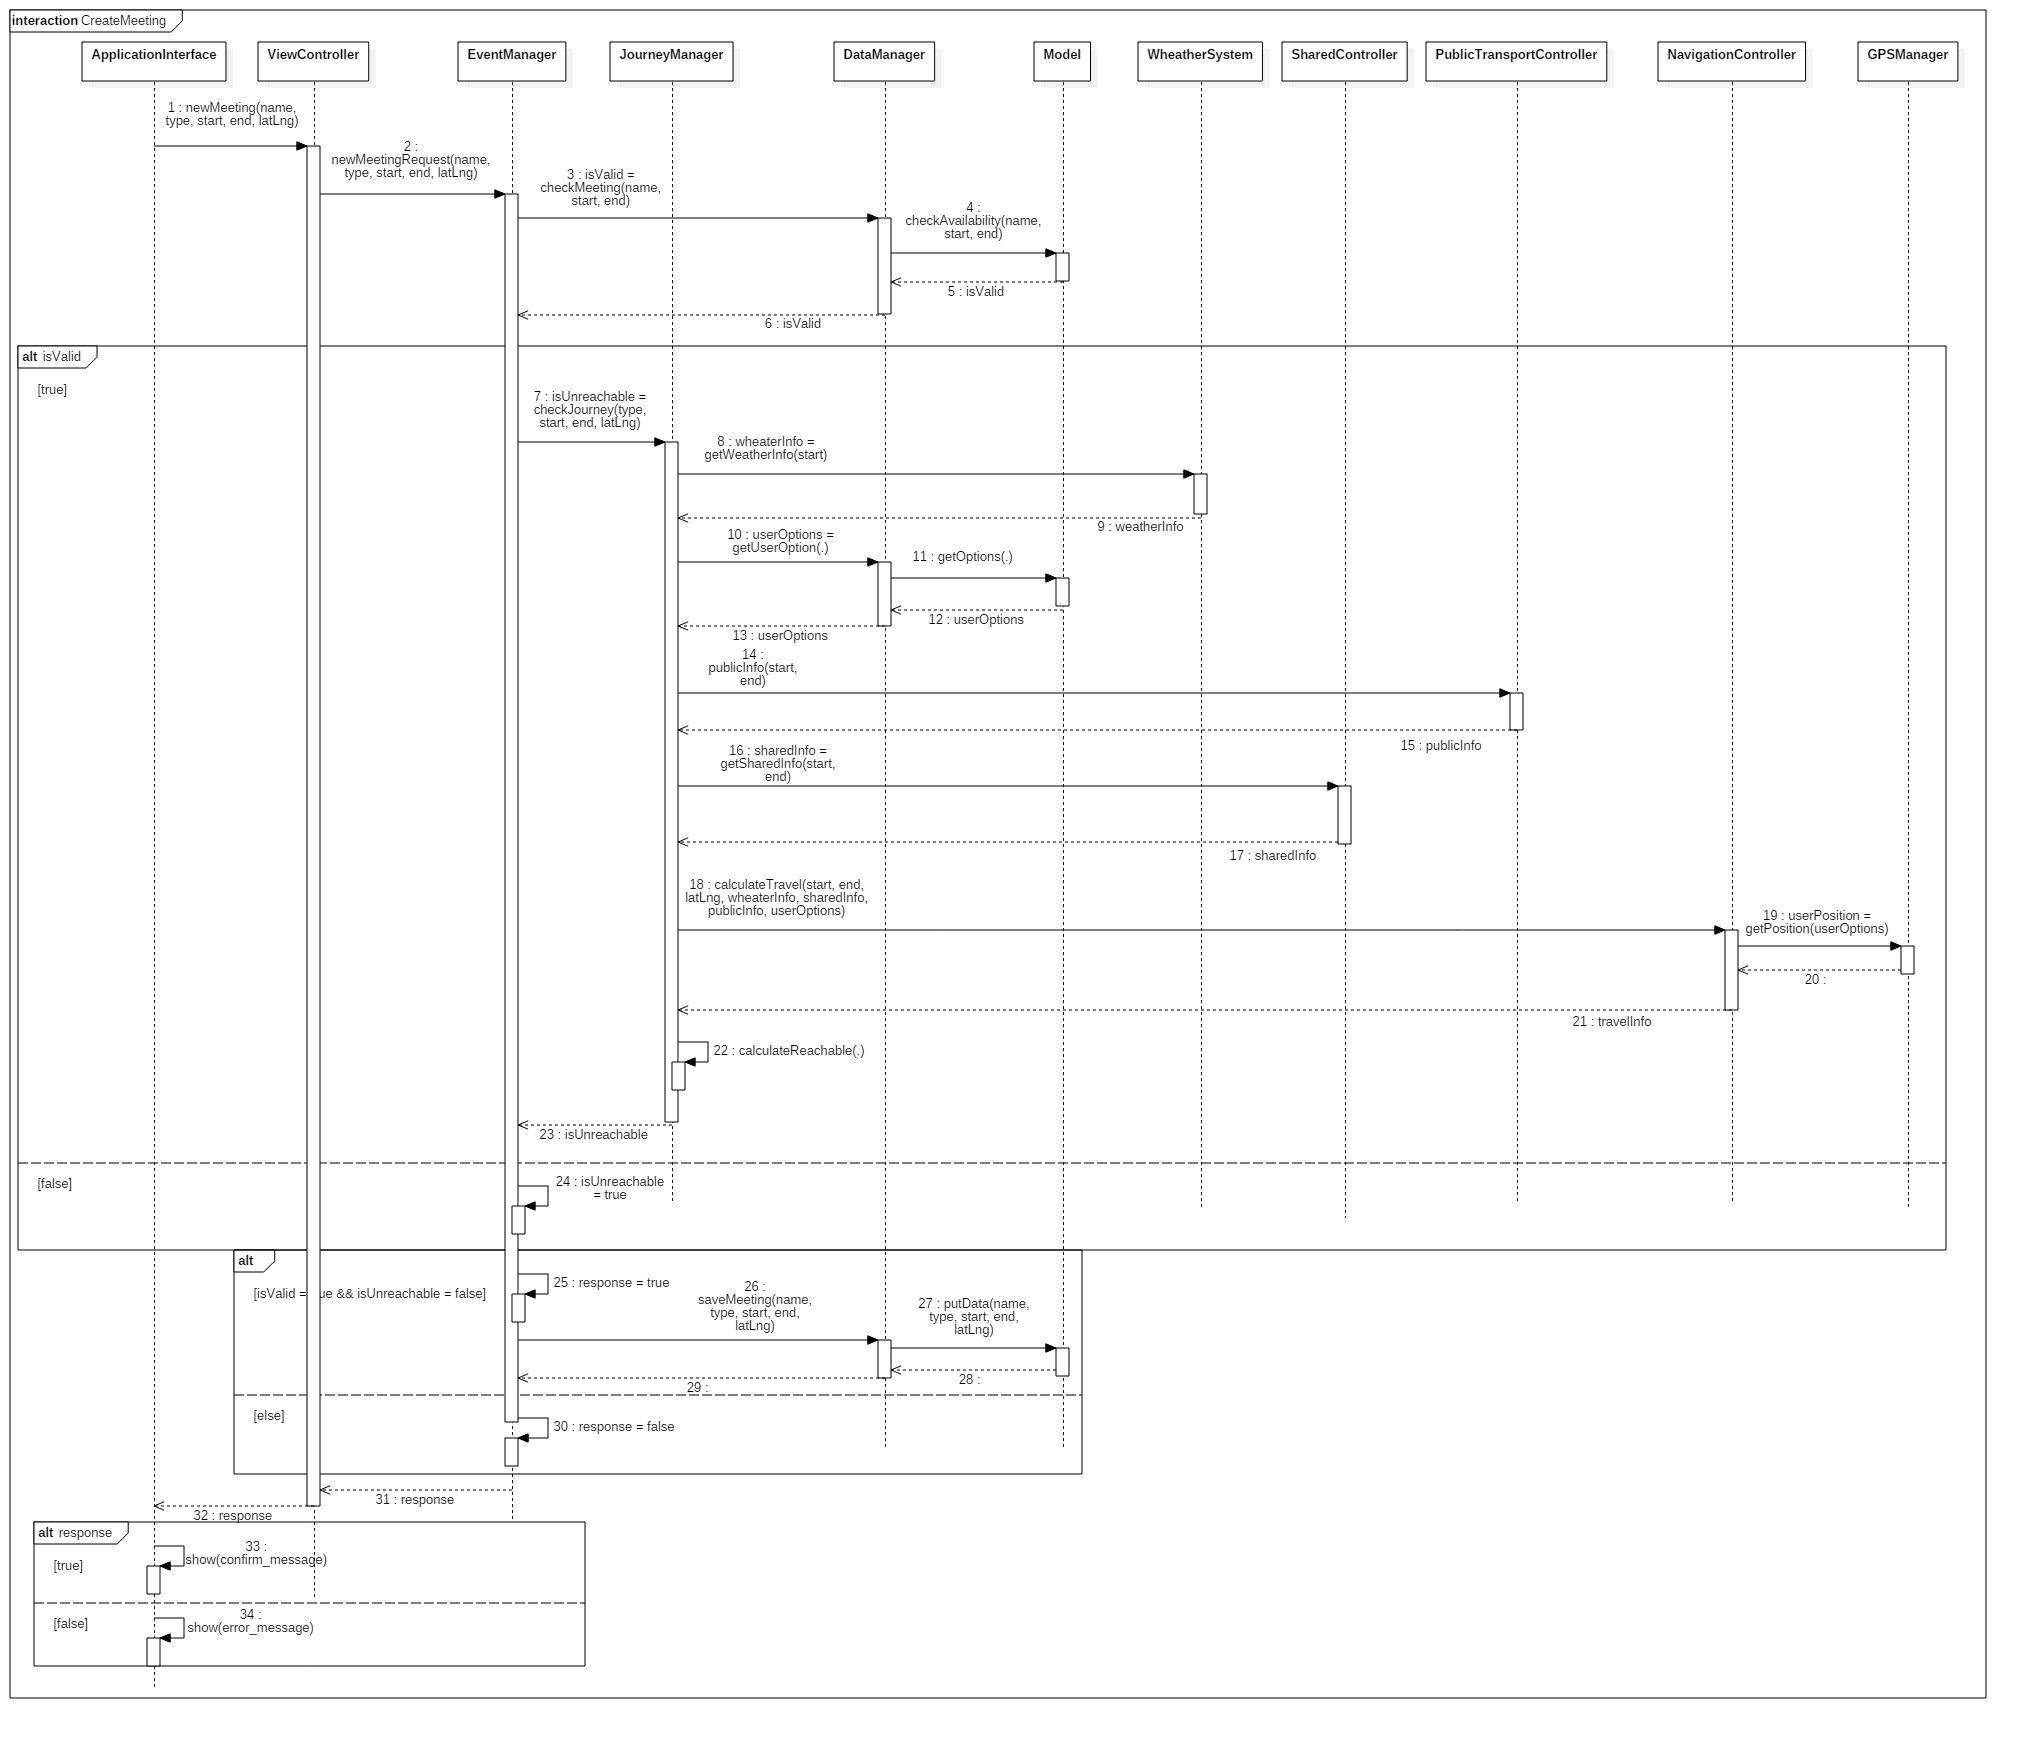
\includegraphics[scale=0.25]{images/CreateMeeting}
\caption{Create Meeting}
\end{figure}This diagram shows the process to create a meeting by using the application. As usual the ApplicationInterface retrieves all information about the meeting that the user wants to create and pass them to the ViewController that call the EventManager component.The EventManager checks in the Model if the name already exists and if the new event has an overlap with an other event. If this is the case the event is defined not valid and the system sets the unreachable of the event. In the other situation the event is valid and the EventManager goes to check the reachability of the event. For check this, the JouerneyManager calls different components to retrieve informations that it needed; the WheaterSystem for weather information, the DataManager and the Model for the user’s options, the PublicTransportController for all informations about hours and availability of public transportations, the SharedController for all information about shared vehicle systems. After that the JourneyManager can call the NavigationController to calculate the travel in base of all informations that it has retrieved earlier. The NavigationController uses the GPSManager for location informations and returns the travel info to the JourneyManager that calculates the reachability of the event in base of the others event that the user has in his Model. Finally if the event is valid and reachable the EventManager save the meeting into the Model and return a response for the ApplicationInterface that show a confirm or an error message based on the received response.

\subsubsection{Travel to the Meeting}
\begin{figure}[H]
\centering
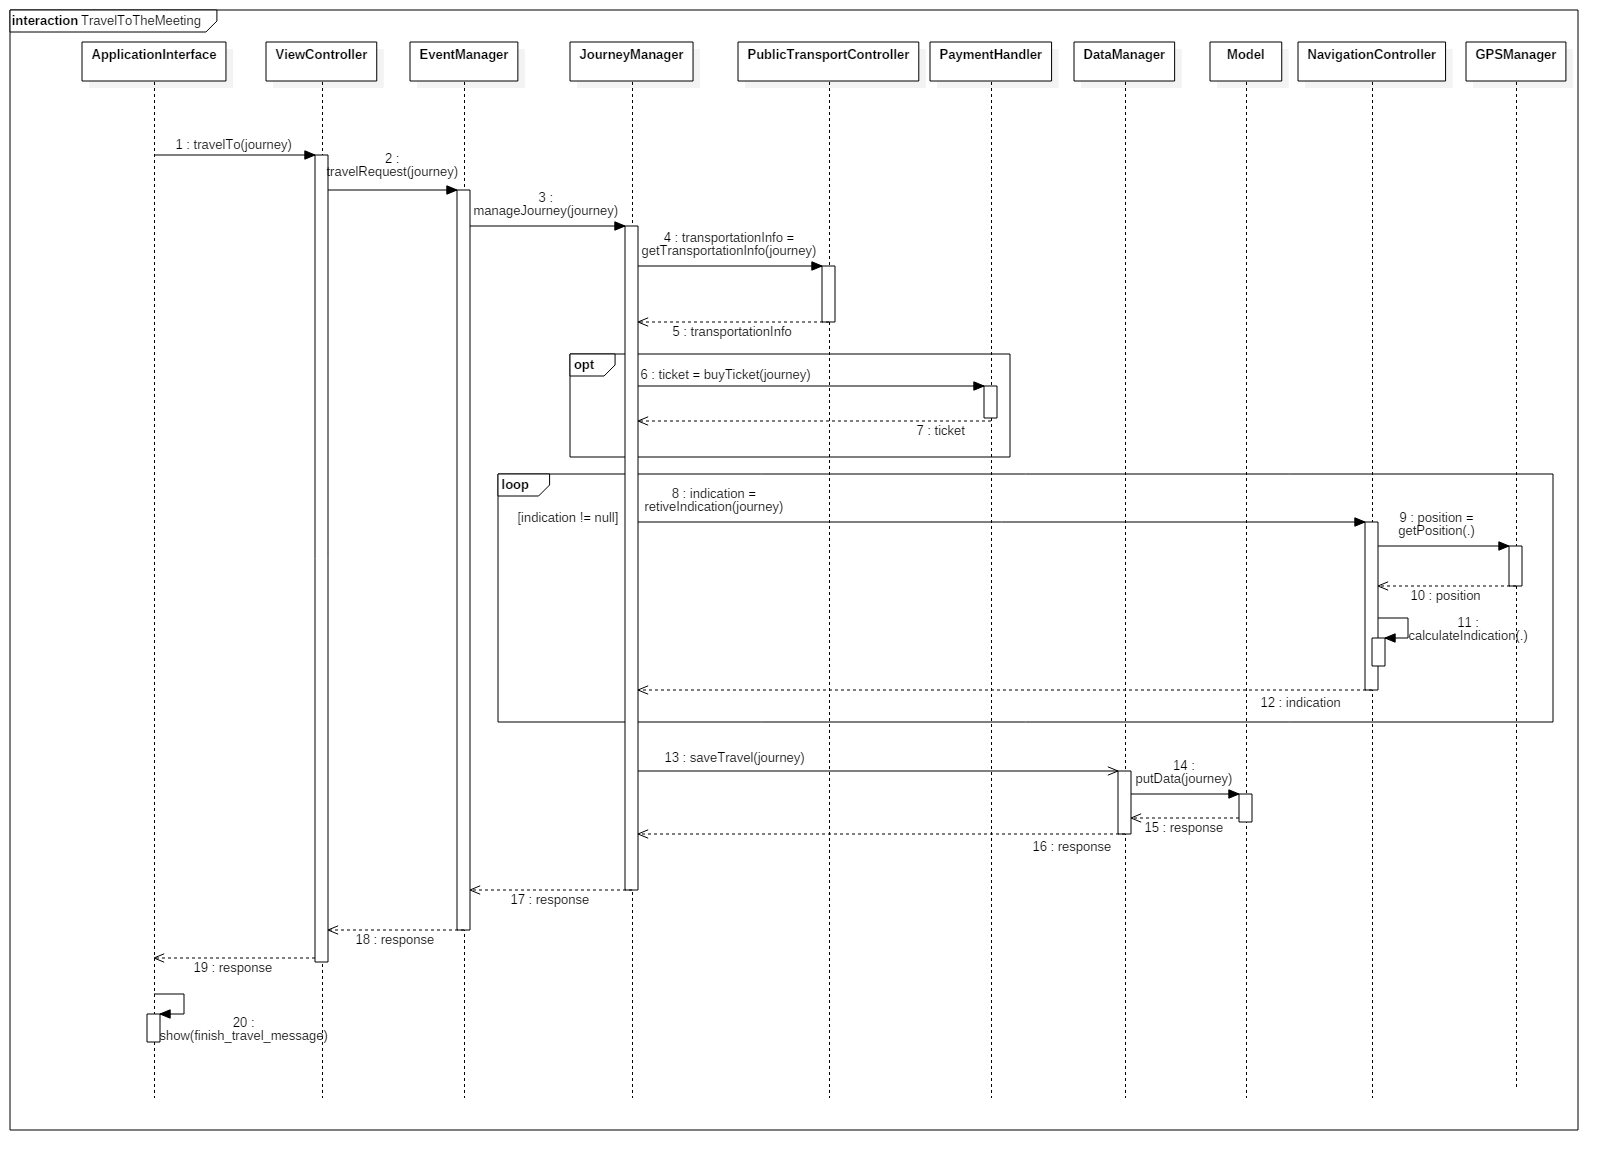
\includegraphics[scale=0.25]{images/TravelToTheMeeting}
\caption{Travel to the Meeting}
\end{figure}In this diagram you can see the travel to a meeting using a public transportation mean. The user starts the navigation in the ApplicationInterface that passes the relative journey to the JourneyManager passing by the ViewController and the EventManager. The journey manager request to the PublicTransportController the information of this journey. In that situation the user has the possibility to buy the ticket for public transportation by using the PaymentHandler. The JourneyManagar retrieve the indication by calling the NavigationController that uses the GPSManagar to take the position of the user, furthermore the NavigationController calculate the indications and returns these to the JourneyManager. The travel is saved into the Model and the ApplicationInterface show a dialog when the travel is finished.

\clearpage
\subsection{Component Interfaces}

\clearpage
\subsection{Selected Architectural styles and patterns}
The following architectural styles have been used:
\begin{itemize}
\item
\textbf{Model-Control-View:} It is used for the main components of the system. It’s a really good choice of design that allows to keep clear the role of every component and that makes the system easier to deploy and maintain.
\item
\textbf{Client-Server:} This pattern is a good practice for a distributed system. It is used between the application server (client) queries the DB (server) and the application (client) communicates with the application server.
\item
\textbf{Service-oriented Architecture:} It is used by the system for the communication between the server and the user’s device (RESTful). The SOA allows to think at a higher level of abstraction, by looking at the component interfaces and not at their specific implementation. SOA style also improves modularity: by making service description, discovery and binding explicit, it is easier to build new plugins and test single modules independently.
\item
\textbf{Fat Client:} The fat client paradigm is implemented because the interaction between user’s device and the server hasn’t a central role in the system behavior . Having a fat client in our case is an advantage because most application logic is on the user’s device, which has sufficient computing power and is able to manage concurrency issue efficiently.
\end{itemize}
